%%%%%%%%%%%%%%%%%%%%%%%%%%
% MSc Project 
% University of Sheffield
% September 2017
%%%%%%%%%%%%%%%%%%%%%%%%%%


\documentclass[11pt,oneside]{book}
\usepackage[margin=1.2in]{geometry}
\usepackage{setspace}
\usepackage[toc,page]{appendix}
\usepackage[none]{hyphenat} % turn hyphenation off by default
\usepackage{graphicx}

\begin{document}

\frontmatter

\begin{titlepage}

% You need to edit the details here

\begin{center}
{\LARGE University of Sheffield}\\[1.5cm]
\linespread{1.2}\huge {\bfseries Lip reading for song transcription}\\[1.5cm]
\linespread{1}

\includegraphics[width=5cm]{images/tuoslogo.png}\\[1cm]
{\Large Xinghui He}\\[1cm]
{\large \emph{Supervisor:} Dr Jon Barker}\\[1cm]
\large A report submitted in fulfilment of the requirements\\ for the degree of MSc in Advanced Computer Science\\[0.3cm] 
\textit{in the}\\[0.3cm]
Department of Computer Science\\[2cm]
\today
\end{center}

\end{titlepage}

% -------------------------------------------------------------------
% Declaration
% -------------------------------------------------------------------

\newpage
\chapter*{\Large Declaration}

\setstretch{1.1} % set the line spacing differently if you wish, but this looks good to me. 

All sentences or passages quoted in this report from other people's work have been specifically acknowledged by clear cross-referencing to author, work and page(s). Any illustrations that are not the work of the author of this report have been used with the explicit permission of the originator and are specifically acknowledged. I understand that failure to do this amounts to plagiarism and will be considered grounds for failure in this project and the degree examination as a whole.\\[1cm]

\noindent Name:\\[1mm]
\rule[1em]{25em}{0.5pt}

\noindent Signature:\\[1mm]
\rule[1em]{25em}{0.5pt}

\noindent Date:\\[1mm]
\rule[1em]{25em}{0.5pt}

% -------------------------------------------------------------------
% Abstract
% -------------------------------------------------------------------

\chapter*{\Large \center Abstract}

Lip-reading for song transcription is a specific topic on the research of visual automatic speech recognition in music. In a traditional dialogue, people recognize the speech content through their auditory sense, visual sense and also according to the circumstances with their own knowledge reserves. If compare audio recognition system to auditory sense, compare video recognition system to visual sense, compare language model to the circumstances, and compare lexicon to knowledge reserves, computer machine also can achieve the ability of recognizing the dialogue by huge training. It is a process of developing an audio-visual automatic speech recognition system. 

But for this project on song transcription, it extends an MSc project that ran last year called ‘Automatic Speech Recognition in Music’\cite{Reference1}. This year we will focus more on the visual front end design in ASR system and compare its performance with last year's audio-only ASR system. The visual-only ASR system would be trained with  traditional GMM-HMM methodologies. Since the experimental results are even more bad than last year's 91.60 percent WER with 98.49 percent WER,  more information on audio-visual fusion would be covered in our paper to prepare for the future's developing on AV-ASR system in music.



% -------------------------------------------------------------------
% TOC etc
% -------------------------------------------------------------------

% -------------------------------------------------------------------
% Acronyms 
% -------------------------------------------------------------------

\chapter*{\Large \center Acronyms}

AAM        \     Active Appearance Model\\
ASM        \     Active Shape Model\\
ASR        \     Automatic Speech Recognition \\
AV-ASR     \     Audio-Visual Automatic Speech Recognition\\
CNN        \ Convolutional Neural Network  \\
DCT       \  Discrete Cosine Transform\\
DFT      \   Discrete Fourier Transform \\
DNN       \  Deep Neural Networks \\
FFT      \   Fast Fourier Transform \\
GMM       \  Gaussian Mixture Model \\
HMM       \  Hidden Markov Model\\
LDA       \  Linear Discriminant Analysis\\
LSTM      \  Long Short-Term Memory\\
MFCC      \  Mel Frequency Cepstral Coefficients \\
MLLT      \  Maximum Likelihood Linear Transformation\\
PCA       \  Principal Component Analysis \\
RNN       \  Recurrent Neural Network\\
SAT       \  Speaker Adapt Training\\
WER       \  Word Error Rate \\


% -------------------------------------------------------------------
% TOC etc
% -------------------------------------------------------------------


\tableofcontents
\listoffigures
\listoftables

\setstretch{1.1} 

\mainmatter

\chapter{Introduction}
Lip-reading is a technique of understanding speech by observing people's lip movement. And lip-reading recognition technology is a technology that integrates machine vision with natural language processing since it contributes to let machine understand language by analyzing speaker’s lip movement. As a simple experiment in psychology called McGurk effect\cite{Reference2} highlighted, auditory sense and visual sense are interacted during the process of recognizing voice. Therefore, it is reasonable to combine audio information with visual information to recognize speech. Due to the huge potentialities in applications like hearing aids or speech recognizer of silent videos and so on, researches on machine lip-reading are emerging in an endless stream nowadays. However, researches on lip-reading in music are still a barely analyzed part in visual automatic speech recognition. 

For mankind, singing is an artistic way to express speech, and music is an artistic product of expressing minds. For ASR, recognition in music is more difficult since the same word has various expression in different songs even when regardless of amateur singer's accent, which may conclude different pronunciation of phoneme in our system's lexicon dictionary, CMUdict\cite{Reference3}. Moreover, the sound of instrument in song's background also increase the coefficients of difficulty in recognizing. Therefore, it is necessary to take advantage of visual information to recognize the speech. And in this project, we would build an visual-only ASR system in music to see whether its performance is better than audio-only ASR system. However, only use visual information would also easily get bad lip reading\cite{1} and the method of extracting visual features affect a lot on our GMM-HMM based system's evaluation. For human, using hearing together with vision is easier than using either of them only to understand the speech. 


\section{project content}

As the paper title ' lip-reading on song transcription' shows, this project would cover more researches on the visual-only ASR system in music. These can be divided as 3 main topics:  audio and video feature extraction,  music corpus construction and how ASR systems implemented with Kaldi\cite{Reference4}, a popular speech recognition toolkit.  In the feature extraction step,  it would refers to what feature to extract and how this feature can be extracted. And in step of  music corpus construction, it would basically to state details about corpus file distribution in our system and the rules of extending the corpus, which designed by Gerardo Roa Dabike\cite{Reference1}. And then,  this paper would also refer to some details of system experiment in Kaldi.  At last, a chapter on analyzing the experimental results and conclusion on our project would be followed.

\section{Aims and Objectives}
Aiming to compare the performance of  Audio-only ASR system with visual-only ASR system, this project would focus on the visual front end design to build an visual-only ASR system with the same music database last year.  In our project, we would train mono-phone and tri-phone acoustic model with audio and visual feature individually and decode them with different n-gram size language model. According to the experimental results, we would see what kind of acoustic model and what size of n-gram language model would be the best choice for audio-only ASR system and visual-only ASR system respectively by comparing their WER. However, both the noise of instrument in audio the quality of ROI in video frames need to be considered as factors that affect the audio and video feature extraction individually. For they both have drawbacks in ASR of music. In the future,  we will adapt the “early” level feature fusion to combine audio and video streams and convert them into Kaldi format in order to combine the audio with video into an AV-ASR system to see its performance. 
 



\chapter{Literature Survey}

Automatic Speech Recognition on music is a barely topic, since the applications on it are mostly for entertainment. Moreover, even though the research of ASR on music are small in quantity, most of them focus mainly on lyrics alignment not lyrics transcription over last decades. However, the continuous researches on music transcription come out since 2010, published by Messaros and Virtanen\cite{Reference5}. 
In terms of lip-reading, the first end-to-end model in the world based on Neural Networks called LipNet\cite{Reference6} comes out in 2016. It maps a variable-length sequence of video frames to text that called sentence-level lip-reading. No one can deny that it is am important breakthrough in lip-reading.
And when it turns to lip-reading for song transcription, the materials that we can find are less. In order to have a basic understanding on how to build an AV-ASR system for song transcription, this Chapter would cover the literature survey on three main component : the methods of extracting audio and video features, two kinds of classification methods (GMM-HMM basically and DNN) and HMM-GMM based ASR system in music. At last, the issues on datasets and a chapter summary are also following concludes.

\section{Feature Extraction }

Feature extraction is a vital stage in our HMM-GMM based ASR systems. To extract useful feature, we avoid any meaningless features, repeated features and complicated features in principle. And try to find a suitable set with the least dimensional feature vectors to achieve the best estimation. Because low dimensional data consumes less machine computing time and also simplifies the training model. If we get a lot typical feature vectors and train a very complicated model, the training error would decrease on training set. But for the testing error, it would increase along with the rise of the complexity of training models. Therefore, how to extract feature and what kind of feature to extract has a fatal impact on system evaluation.
And in this section, we will emphasize the process and methods of extracting both audio and video features.

\subsection{Audio Feature Extraction}
This section is to describe how to get the acoustic feature factors that transformed from the input waveform. And in this feature extracting process, we would particularly make research on MFCC \cite{Reference7}(the mel frequency cepstral coefficients, a widely used feature representation in speech recognition) and use scripts in Kaldi to realize to get the feature vectors. And here is the figure \ref{fig:mfccpro} to describe the extracting process.
\begin{figure}[ht]
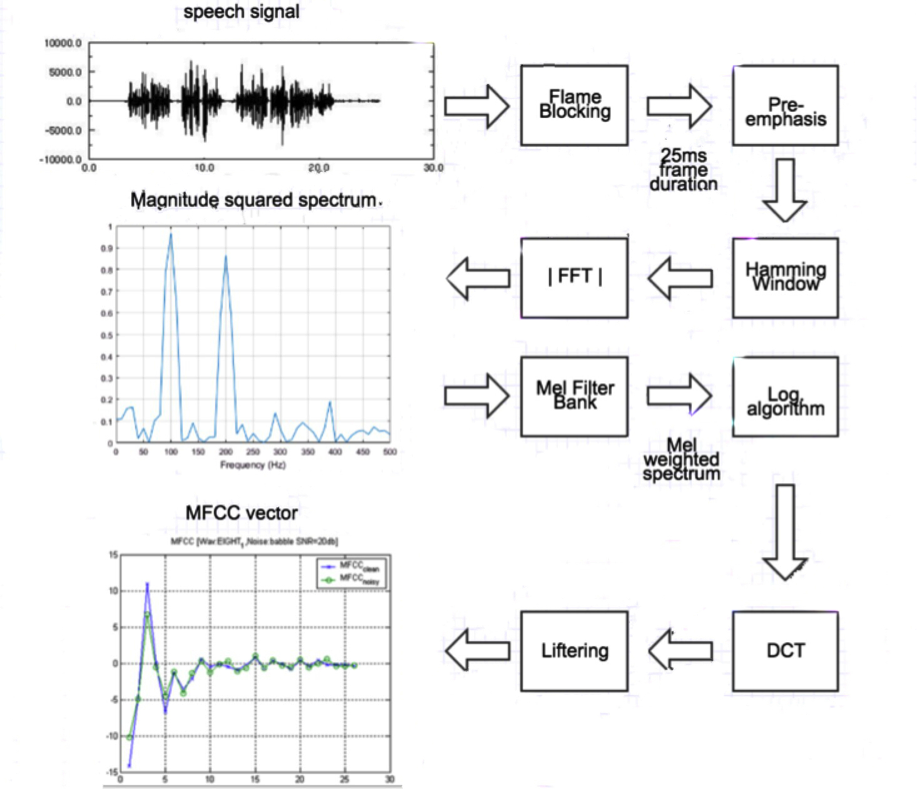
\includegraphics[width=1\linewidth]{figures/extractmfccprocess.png}
\caption{the process of extracting mfcc feature vectors}
\label{fig:mfccpro}
\end{figure}


As the figure shows above, we can conclude the process of extracting mfcc feature vectors into several steps:
\begin{enumerate}
\item Sample and quantize the speech signal into digital waveforms.
\item Frame blocking typically 25 ms frames duration with 10ms shift.
\item Boost the waveforms’ energy in the part of high frequencies by using a high-pass filter. 
\item Use Hamming window to make frames continuous for Fourier analysis.
\item Adapt FFT algorithm to compute the DFT in order to get the spectrum from hamming-windowed signal.
\item Collect energy from each frequency band by Mel filter bank and get fbank feature.
\item Compute the log of the spectrum values in each Mel bin.
\item Take the DCT and keep as many as MFCC coefficients.
\item Do cepstral liftering to scale the range of coefficients.
\end{enumerate}
In this way, we can get standard cepstral vectors of audio. To extract dynamic mfcc features, we do delta function on mfcc to get the velocity of feature changes. Besides, if we adapt delta-delta function on mfcc, we can get accelerated velocity of feature variation .



\subsection{Visual Feature Extraction}
Visual feature can be divided as appearance-based pixel feature and shape-based feature. And in our visual-only ASR system, we use the ensemble regression tree method\cite{Reference8},which is implemented in dlib toolkit to extract histogram of oriented gradients feature\cite{Reference9} in order to detect facial 68 landmarks feature. And then we extract the according to the lip region landmarks. Here the histogram of oriented gradients feature is shape-based feature, while lip region pixel feature is appearance-based pixel feature.

Nowadays, the methods of extracting video features are mainly based on pixels or models. And this section would focus on means of models, especially on the literature of ASM and AMM, since they have been proved more informatively and visually on extracting facial features with flexible and repeated geometrical characteristic.

\subsubsection{Active Shape Models}
Active shape models (ASMs)\cite{Reference10} are statistical models of the shape of objects, which aims to fit an example of the same object in a new image by iteratively deform. ASMs are models generally consist of two parts: A Point Distribution Model and a set of Local Gray-Level models. The former part uses object’s landmark points to model the shape and its variants. Besides, the latter part is used to capture the local gray-level variants at each landmark points. 

ASMs are also flexible models to represent the shape and appearance of faces in images. It uses Principal Component Analysis\cite{Reference11} (PCA) to learn a generic model from the facial landmarks in training data, and then fits the best match target points in test data, typically by some greedy searches.

Here are also some ASM fitting result \ref{img:ASM1} show below, which gets by initializing an approximate fit to the training data, and then updating the parameters (Xt, Yt, s, θ, b), applying constraints to them and repeat until convergence.

\begin{center}
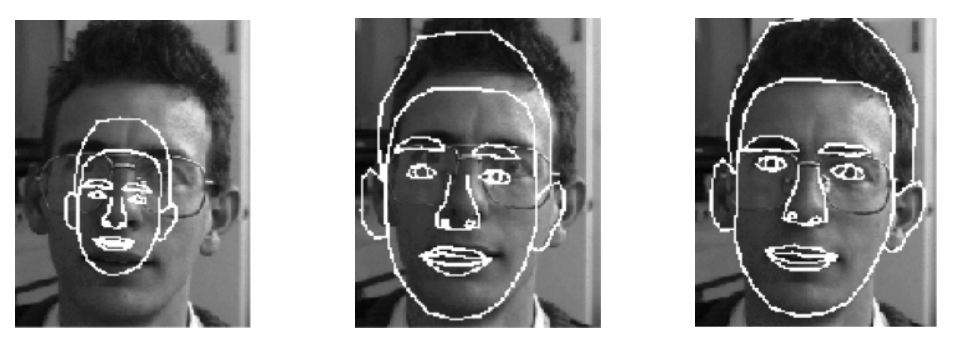
\includegraphics[width=0.8\linewidth]{images/ASM1.png}\\[1cm]
\label{img:ASM1}
\end{center}

\subsubsection{Active Appearance Model}


An active appearance model \cite{Reference12}(AAM) is a computer vision algorithm combined a statistical shape model with a texture model that aims to match a set of object shape and appearance to a new image. It is related to the ASM, since they have similar process to build models from training phrase. The difference is that the ASM seeks to match model points, while the AAM seeks to match not only the model points but also a representation of the texture of the object in an image. Therefore, the AAM can be considered as an extension of the ASM approach and be used in object detection widely nowadays. In our project, we can use tools like dlib or openCV to get the object’s shape and texture information in image, and then fits the best match model in testing data, typically by some greedy searches. 

Compared with ASM,our project is more reasonable to adapt AAM,since it learns model from both shape and texture information, while sometimes singer does not face to the camera. As a result, tools may be not get the landmarks. Problems get solved when adapting AMM rather than ASM.

Applying PCA, we can model the statistical variation with formula below.
        
        A shape model:
        \begin{equation} X=\bar{X}+P_{s}b_{s}\end{equation}
        A texture model:
        \begin{equation}  g=\bar{g}+P_{g}b_{g}\end{equation}
        A shape and texture combined model:
        \begin{equation}  
       b=\begin{pmatrix}
W_{s}b_{s}\\b_{g}
\end{pmatrix}=\begin{pmatrix}
W_{s}P_{s}^{T}(x-\bar{x})\\ P_{g}^{T}(g-\bar{g})
\end{pmatrix}
        \end{equation}
        
Here are some examples to show the AAM fitting result\ref{img:AAM1}.
\begin{center}
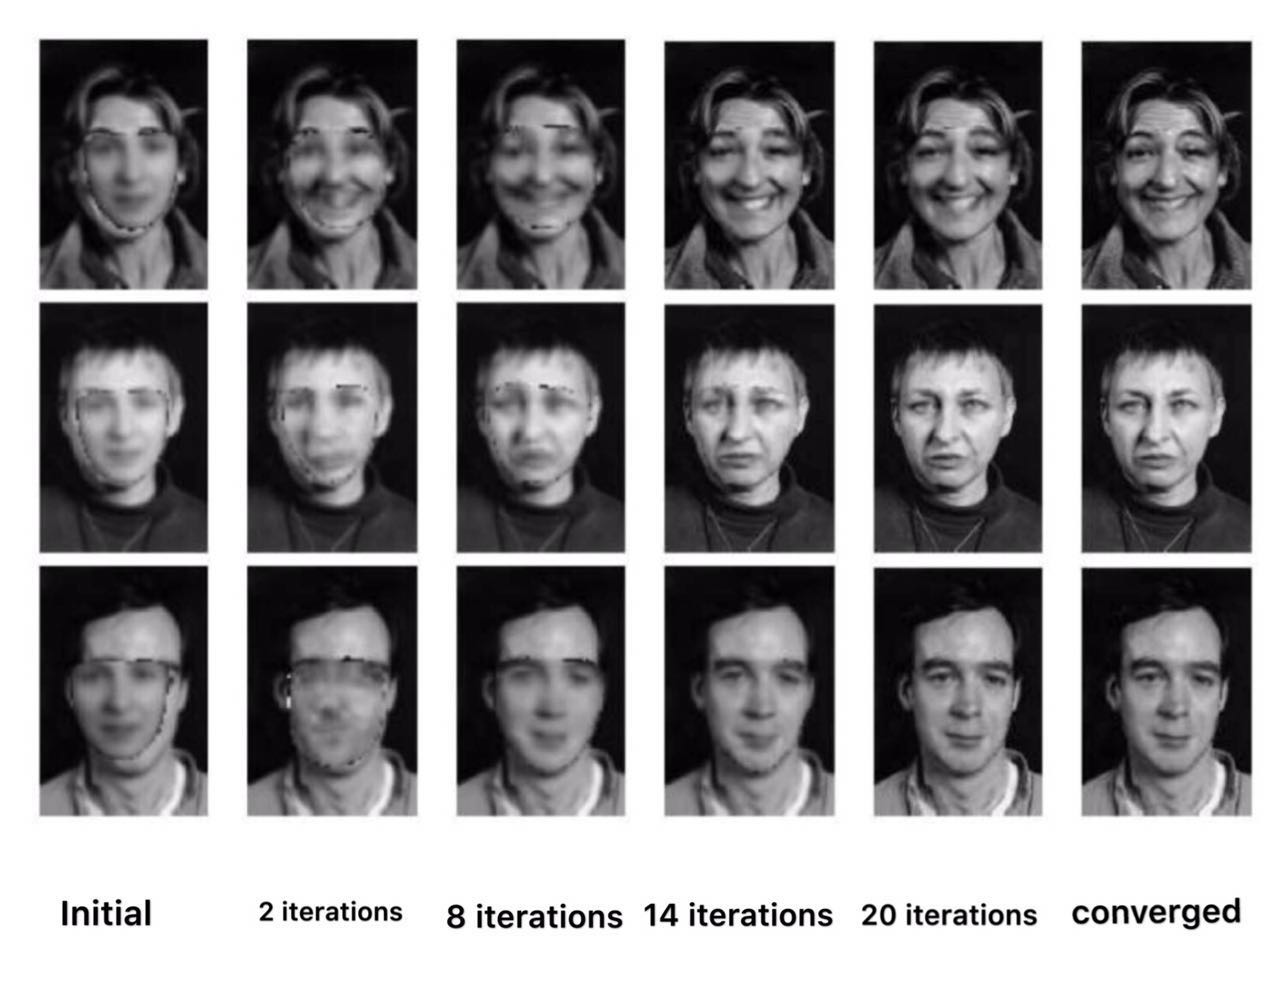
\includegraphics[width=0.8\linewidth]{images/AAM1.jpeg}\\[1cm]
\label{img:AAM1}
\end{center}

\subsubsection{Audio-Visual fusion}
Audio–visual fusion is a major research topic in the process of building an AV-ASR system, which aims to combine video with audio streams into a bimodal classifier. The video streams are usually starts early than audio streams, for example when the lip starts to move, the voice still not come out. Since the two streams are not perfectly synchronous with each other, the AV-fusion is complicated.

Basically, we have two methods that can be considered for AV-fusion: feature fusion, decision fusion. Feature fusion is considered as an “early” level fusion method, while decision fusion is a “late” level fusion\cite{Reference13}. Even though feature fusion techniques making work easier in improving ASR over audio-only result, the reliability of each modality cannot be ensured. Therefore, using a weighted decision fusion to develop the AV-ASR system may get better results than using feature level fusion. However, the decision fusion may be more difficult than feature fusion.

\section{Classification}
In this section, we would cover the literature of statistic models, HMM and GMM. They are popular models to be adapted into ASR systems. Since we did not adapt DNN methodologies into our system, the literature on DNN we covered in the chapter is rough. It is for introduction, because using the machine deep learning methodology is the new trend to develop ASR systems.

\subsection{Gaussian Mixture Models}
The Gaussian Mixture Model \cite{Reference14}(GMM) is a most common parametric probability density function by far, which superposed by M component Gaussian densities, to describe the distribution of the dataset.
At the same time, a GMM can be expressed by equation (2.4) in a mathematical way. 

\begin{equation}
p(x|\lambda )=\sum_{i=1}^{M}w{_{i}}g(x|\mu{_{i}},\Sigma _{i} )
\end{equation}

where, \begin{equation}
\sum_{i=1}^{M}w{_{i}}=1
\end{equation}
  (x is a D-dimensional vector data, wi , i = 1, . . . , M, are the weights for every single Gaussian function)
The shape of Gaussians controlled by the mean and unit variance,  
Gaussians have the same shape, with the location controlled by the mean, and here is the figure \ref{fig:gmm} to show the shape of one-dimensional Gaussians with different mean and variance.

\begin{figure}[ht]
\centering
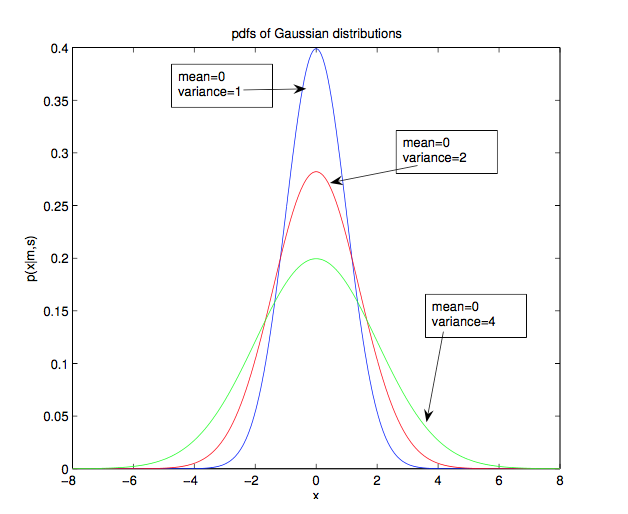
\includegraphics[width=0.5\linewidth]{figures/gmm.png}
\caption{pdfs of Gaussian distributions[7]}
\label{fig:gmm}
\end{figure}

  
  
  
\subsection{Hidden Markov Model}
The Hidden Markov Model \cite{Reference15}(HMM) is a popular statistical tool in process of speech recognition, since it can model a wide range of time series data and work on both audio and video frames. We use HMM in this project, which aims to recognize the extracted audio and video features as a series of HMM state. 


\begin{figure}[ht]
\centering
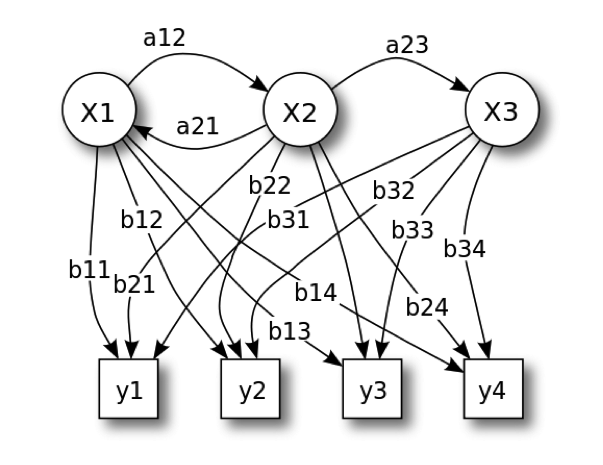
\includegraphics[width=0.5\linewidth]{figures/hmm.png}
\caption{Probabilistic parameters of a hidden Markov model}
\label{fig:hmm}
\end{figure}



As the figure \ref{fig:hmm} shows above, a HMM is composed by a sequence of states (x) that generates a sequence of emissions (y). And for states, there is a GMM probability density function (b) associated with each of them and also a transition probability (a) between them.  In addition, we can apply some basic training algorithms in HMM for maximum likelihood estimation to get the emissions. For Viterbi Algorithm\cite{Reference16}, it can be used to find the most likely path of getting the emissions without problems of hidden states. And for Forward Algorithm, we use it to compute the probability of the observation sequence after a given HMM. Besides, a combined version, forward-backward algorithm (Baum-Welch algorithm), can be adapted to estimate a most suitable HMM according to observed emissions with a related set of hidden states.

\subsection{Deep Neural Networks }
The neural network is a set of algorithms designed for mimicking the way that human brain works. Different with traditional machine learning algorithms, it can automatically extract features from unstructured data like audio and video frames and then cluster and classify them. Any particular Neural Networks like RNN or CNN are superposed by multiply layers while each layer composed by neural unit. Applied with an activation function, here is a figure\ref{fig:nn} shows how a neural unit, which from an input layer xi and weighted by a wi factor, that works.
\begin{figure}[ht]
\centering
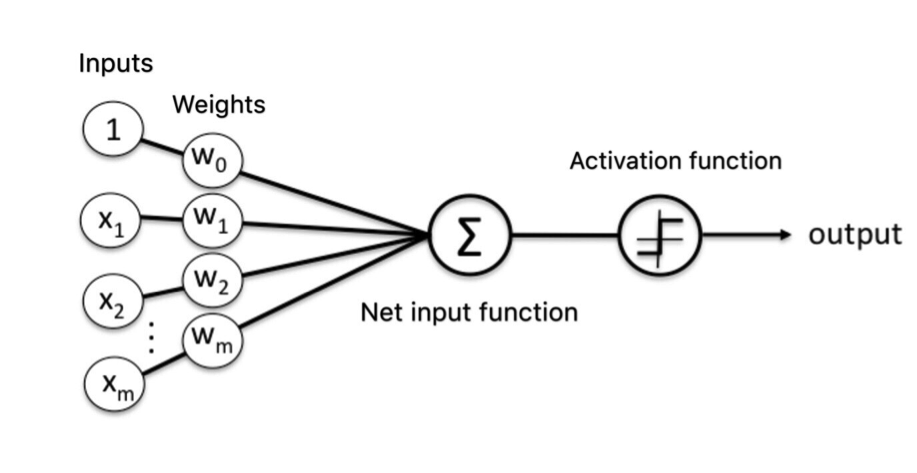
\includegraphics[width=0.5\linewidth]{figures/nn.png}\\[1cm]
\caption{neural unit work in neural networks}
\label{fig:nn}
\end{figure}




Besides, when it comes to DNN, there are at least 3 layers: input layer, hidden layer and output layer. Moreover, every layer learns on the basic of the former layer. Therefore, the future recognized by neural unit becomes complicated along with the increasing number of layers. 
Here is an example \ref{fig:dnn} to show the process of successive model layers learn deeper intermediate representations.
\begin{figure}[ht]
\centering
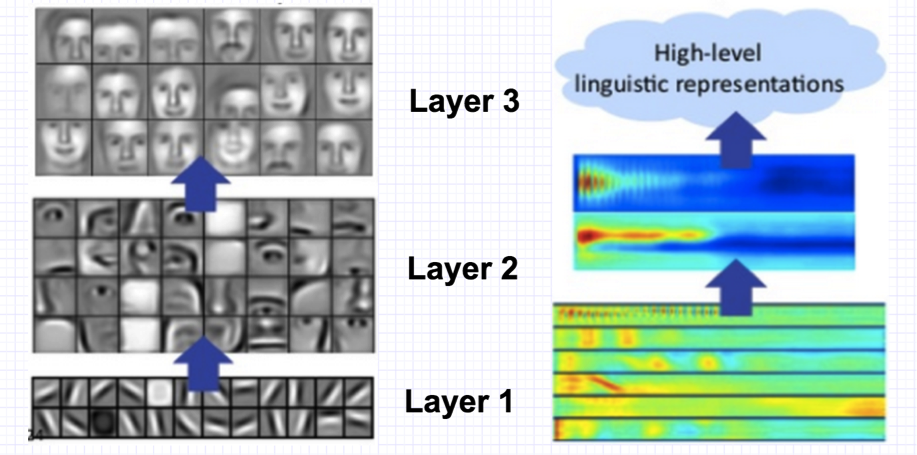
\includegraphics[width=1\linewidth]{figures/dnn.png}
\caption{the process of successive model layers learn deeper intermediate representations}
\label{fig:dnn}
\end{figure}

And to our project, the temporal aspect is important to both audio and video component. As a result, we feed the representation of each audio or video “frames” to a RNN in order to understand the sequential information between them, since a RNN is designed for recognizing sequences.  And especially use LSTM
to propagate and learn to control the informative streams over more time steps with forget gates. What is more, the CNN can be used to describe any individual frame and extract feature from them.

\section{HMM-GMM based ASR system in music}
Automatic Speech Recognition is a task to let machine learn how to convert the input signal into corresponded text.  And in this project, we adapt a traditional HMM-GMM statistic model into our systems. As the picture \ref{fig:hmmgmm} shows, HMM is to describe the dynamism with short-term stationary of states, and GMM describes the feature distribution in every state.
\begin{figure}[ht]
\centering
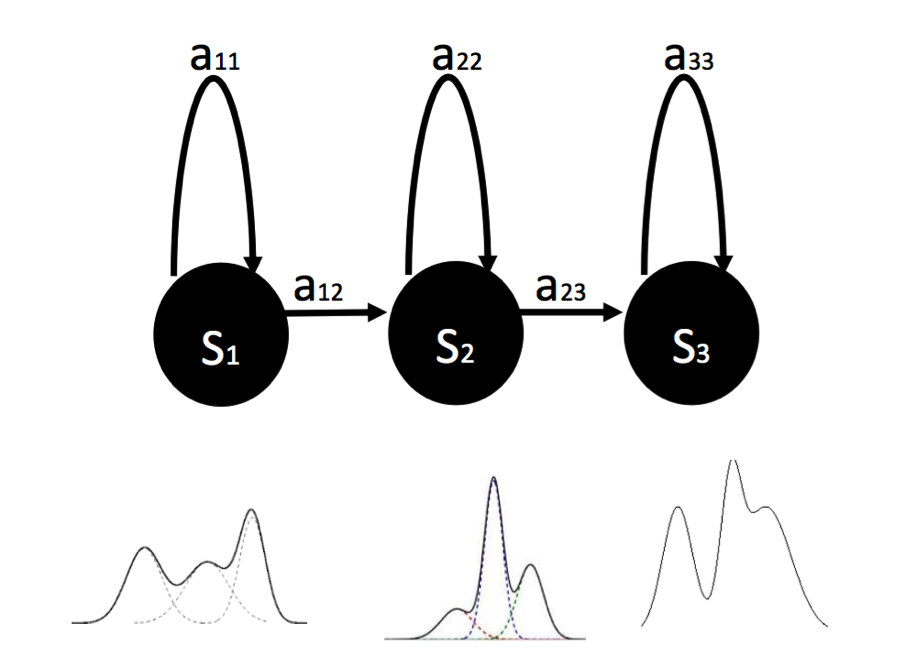
\includegraphics[width=0.5\linewidth]{figures/hmmgmm.png}
\caption{states in GMM-HMM}
\label{fig:hmmgmm}
\end{figure}
HMM-GMM based ASR systems also have mathematic framework of them stated as below: 
        \begin{equation}
        W^{*}=arg max P(W|X)
       =arg max\frac{P(X|W)P(W)}{P(X)}
       =arg max P(X|W)P(W)
        \end{equation} 
        
W represents transcription and X represents the input signal. For X is the input signal, it is hard to calculate the formula in the first line. Therefore, we adapt bayes formula in the second line. And for the input signals are continuous, the equation can be transformed into the third line.  At last, we need to find the most likely transcription W*. The HMM mathematic framework describes the process of an ASR system, w* represents the decode result, P (X|W) represents acoustic model and P (W) represents the language model. 
Moreover, words can be divided into sequences of HMM states Q. 
           
\subsection{Acoustic model}    
Refers to the equation above,the task of acoustic model is to compute P(X|W). No matter in audio ASR system or video ASR system, we both need to adapt their features to train acoustic models. In this project, we would train mono phone acoustic model and tri-phone acoustic model and compare their performances. 

As the figures \ref{fig:wsm} show below, the process of training acoustic models is to model the phones with HMMs, and the states of phones are presented in normal distribution. The system would update the parameters of HMM and GMM by iterated training.
        
\begin{figure}[ht]
\centering
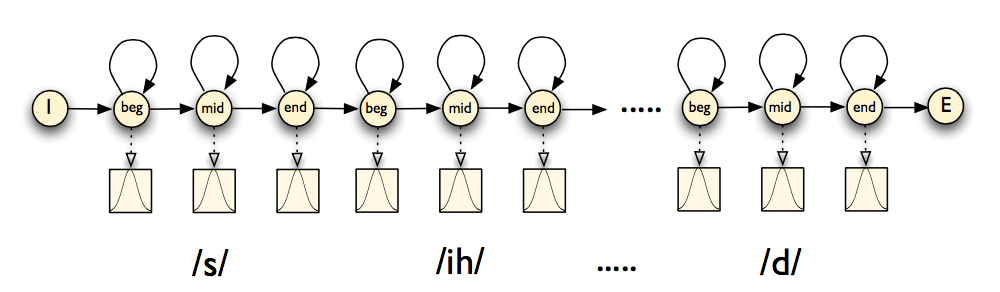
\includegraphics[width=1\linewidth]{figures/wsm.png}
\caption{'six quid' Word sequence models}
\label{fig:wsm}
\end{figure}

\subsection{Language model}
The language model represents the prior probability of the word sequence P(W) and is used for disambiguating between similar acoustics. For example, ‘ I want to see/sea ’. ‘Sea’ has the same pronunciation with ‘see’, but ‘I want to sea’ does not match the grammar rules.
And in speech recognition, language model are statistical model and usually be called as n-gram language model. On average, bigram is the most popular size of language model implemented in ASR system. However, it depends by different system’s database and would affect the system’s evaluation. We should decide the n-gram size by comparing system’s result. 

\subsection{Decode ASR systems}
In HMM-GMM based ASR systems, the developing process is mainly divided into 3 steps: feature extraction, classifier training, and decoding. Since the former two topics already been covered in former sections, this section is going to refer to the topic of decoding our ASR systems.
To show it clearly, here is the figure \ref{fig:aasr} and \ref{fig:vasr} to show the systems construction.
\begin{figure}[ht]
\centering
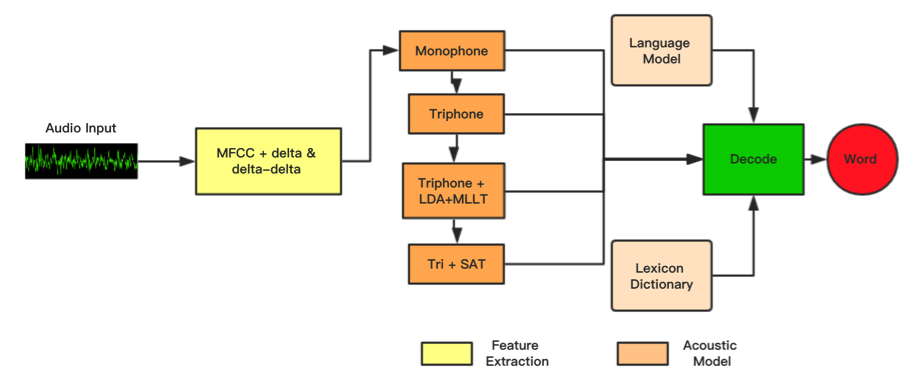
\includegraphics[width=1\linewidth]{figures/aasr.png}
\caption{audio-only ASR system construction}
\label{fig:aasr}
\end{figure}
\begin{figure}[ht]
\centering
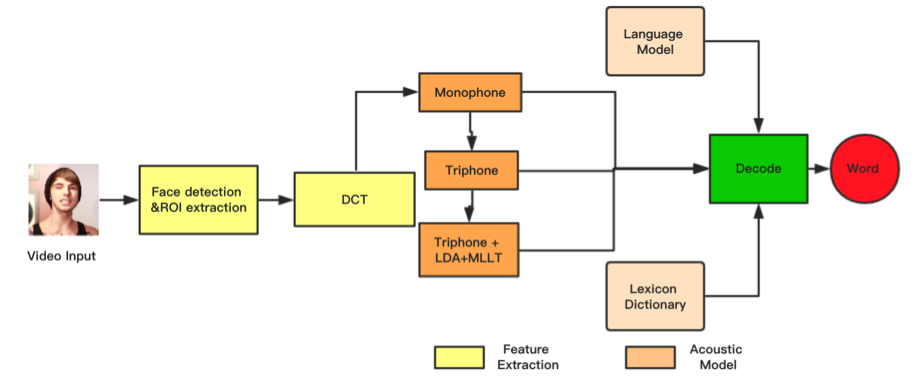
\includegraphics[width=1\linewidth]{figures/vasr.png}
\caption{visual-only ASR system construction}
\label{fig:vasr}
\end{figure}

In our system which is implemented in Kaldi, it would use OpenFst library to let all the resources of language model, acoustic model and grammar files are presented into fst format and generate decoding graph from them. At last, use viterbi algorithm to search the most likely path. 

\subsection{Dataset}
\subsubsection{Speech Database VS Singing Database}
Speech database is a database that concludes speech audio files and text transcription, while singing database composed by singing audio files and lyrics transcription. The singing voice is an artistic expression of speech voice spoken by singer, carrying with more information on musicality. While the speech voice tends to focus on completing the spoken word. On the other hand, the speech voice is flexible to change the pitch and loudness. But for singing voice, the frequencies fluctuate in a significantly soft way compared with speech voice. Moreover, the format of transcription between them is obviously different in the scope of topics and grammar. Text transcription may refer to any topics with a wide range and write with complicated grammar. But for lyrics transcription, the topics of it are limited. For example, probably no one would translate a science manuscript into a singing voice, while a speech voice is possible. What is more, the lyrics transcription usually has picky grammar like poems.
Thus, in terms of practicability, speech database are more suitable than singing database for no matter audio-only ASR system or AV-ASR system.

\section{summary}
To conclude this chapter, we mainly refer to the literature survey on the method of feature extraction, classification and components in ASR systems. They are all useful surveys of helping to build our ASR systems with HMM-GMM methodologies. However, to keep up the pace with the Lip-reading development nowadays, we should focus more on studying deep learning method to see whether it would improve the ASR system in music. Because no matter audio-only system or visual-only system is hard to get a good result in music with HMM-GMM methods.
The first end-to-end model, LipNet[8], which is learnt from deep learning methods, comes out last year. This breaking news can be said as a milestone event in the history of lip-reading research and also accelerate the development on these researches. However, even when the researches on lip-reading are emerging nowadays, Lip-reading for song transcription is still a barely analyzed issue. Therefore, this topic still has much space to exploit on it.

\chapter{ACOMUS Database}
The ACOMUS Database is the database we used in our ASR system in music,which is designed by Gerardo Roa Dabike. It concludes 240 English songs covered by amateur singers that are collected from YouTube. Among these songs, 200 songs are accompanied by guitar and the left 40 songs are accompanied by piano. Each song in this database has a unique song id, which composed by information of gender, sequence number of artist and instrument. For example song id:F002\_002\_01\_0101, F002 stands for the information that the second amateur singer in database's singer list is female, the following 002 means this song is the second song in song's list, and o1 represents guitar.
To look through the unique id in database, it is clear to see there are 174 amateur singers and 213 different songs in this database.


\section{ACOMUS2 Corpus}
Acoustic Cover Music Corpus 2 is a collection of isolated audio and video segments of every sentence in the singing parts of acoustic covers from amateur artist extracted from YouTube. The corpus is in English Language and the music has no restriction of style. The audio files are 16kHz sample-rated one channel files in wav format. And video files are in MPEG-4 format.For quality, the audios are accompanied with one instrument typically guitar or piano. Besides, some of the videos have low image resolution and the quantity of useful frames is small.

     
        
\subsection{Lyrics Annotation}
Lyrics is a computer file format that synchronizes song lyrics with an audio file[10]. For this project, we can only generate all the lyrics by hand for that the official lyrics would not match with the covers. We can observe the static lyrics from the website http://lyrics.wikia.com. However, it still need to check with every utterance in covers. Because the acoustic cover is not singer's official song, amateur artist may not follow the original lyrics with every utterance and sometimes they would changes some sentences in the original lyrics. Therefore, we need to modify the original lyrics to match with the cover. Moreover, we still need to segment the songs with individual sentences with methods of marking the time when every single sentence starts and stops and store them into json format in our database firstly. And then transfer them into kaldi format, only in that way it can be read by Kaldi and used in the last stage of ASR system when scoring the WER.   

\subsection{Audio and video files distribution}
As stated in the above section, the process of annotating songs consumes time and energy. In the ACOMUS Database, there are 120 songs been annotated. Even though the accumulation time of annotated songs is already not long for training acoustic models, not all the annotated utterances can be used especially in visual-only ASR system since it is picky to pick up good utterances to extract visual features. Here is the table \ref{tab:utterance} to show distribution of annotated utterances being used in audio-only ASR system and visual-only ASR system respectively.
\begin{table}[ht]
\center
\begin{tabular}{c|cc}
System & quantity of annotated utterances & time size of annotated utterances\\
\hline
A-ASR system & 3428 & 282 min\\
V-ASR system & 1013 & 83 min\\

\end{tabular}
\caption{System distribution of used utterances}
\label{tab:utterance}
\end{table}



\section{Language Model}
In order to generate a suitable language model for our ASR system in music. It is better to collect the lyrics with the similar style of songs in our database. 
Therefore, the language model is based on a lyrics corpus composed by other songs from the same 157 original singer in database. In addition, another 39 popular singers would be appended to our singer's list. At last, the lyrics corpus is generated by 25916 songs from these 196 singers.

\section{Acoustic Model}

The pronunciation of phonemes in our acoustic model is based on CMUdict, a dictionary has 39 phonemes and 133,031 different words. Aiming to keep the model to be simple, only 5000 words are selected from the dictionary. The rules of selecting these 5000 words are to keep as many as words in annotated utterance. However, there are only 3500 words can be generated from our database (among 240 songs). To complete the construction of 5k words, the left 1500 words were generated by random.

Finally, we generated the 5k words and saved it as lexicon.txt according to the annotated utterances.


\chapter{System implementation in Kaldi}
Kaldi is a popular, open-source, speech recognition toolkit that based on weighted finite-state transducers.This chapter is going to describe how Kaldi works to build the AV-ASR system in our music corpus.
\section{Data preparation}

In our asr-music/s5 recipe, some files need to be prepared by hand and get stored in folder asr-music/s5/data, while others can be generated by Kaldi's tools like the table \ref{tab:datafile} below shows.

\begin{table}[ht]
\center
\begin{tabular}{c|c}
files prepared by hand & files generated by Kaldi \\
\hline
utt2spk & spk2utt\\
spk2gender & cmvn.scp\\
text & feats.scp \\
wav.scp &  \\ 
\end{tabular}
\caption{File distribution in prepared data}
\label{tab:datafile}
\end{table}

To know more about what are these data file, here are also some tables to show the format of files prepared by hand.

\begin{table}[ht]
\center
\begin{tabular}{c|c}

utterance-id & speaker-id \\ \hline
F002\_002\_01\_0101.00.001  & F002\_01\\
...\\ \hline
\end{tabular}
\caption{utt2spk format}
\label{tab:utt2spk}
\end{table}

\begin{table}[ht]
\center
\begin{tabular}{c|c}

speaker-id & gender\\ \hline
F002\_01 & f\\
...\\ \hline
\end{tabular}
\caption{spk2gender format}
\label{tab:spk2gender}
\end{table}


\begin{table}[ht]
\center
\begin{tabular}{c|c}

utterance-id & annotation \\ \hline
F002\_002\_01\_0101.00.001  & THIS WAS ALL YOU\\ \hline
...\\ \hline
\end{tabular}
\caption{text format}
\label{tab:text}
\end{table}



\begin{table}[ht]
\center
\begin{tabular}{c|c}

utterance-id & extended-filename \\ \hline
F002\_002\_01\_0101.00.001  & video/mp4\_segments/F/F002/F002\_002\_01\_0101.00.001.mp4\\ \hline
...\\ \hline
\end{tabular}
\caption{wav.scp format}
\label{tab:wav.scp}
\end{table}



\subsubsection{Methods of files generated by Kaldi}
\begin{table}[ht]
\center
\begin{tabular}{ll} \hline
filename & generate tools  \\ \hline
spk2utt & utils/utt2spk\_to\_spk2utt.pl\\ \hline
feats.scp & audio:steps/make\_mfcc.sh \\ \hline
         & video: \\ \hline
         & 1.use extract\_video\_features.py to get utterance-id.lip\_dct.hdf5 \\ \hline
         & 2.convert this hdf5 file into feats.txt with Kaldi's ark format \\ \hline
         & 3.copy-feats ark,t:feats.txt ark,scp:video.ark,feats.scp  \\ \hline
cmvn.scp & steps/compute\_cmvn\_stats.sh\\ \hline
...\\ \hline

\end{tabular}
\end{table}



After get these data prepared, we still need to run utils/validate\_data\_dir.sh to check if anything already prepared well in the data directory. Sometimes it would occur some errors, like 'utt2spk is not in sorted order when sorted first on speaker-id '. Then basically we use utils/fix\_data\_dir.sh to fix it.


\section{Feature extraction}
This section would cover how to extract audio and video features individually and adapt them to be read by Kaldi. 
\subsection{mfcc extraction}
Kaldi’s waveform-reading code can create MFCC and PLP features to do the ASR. 
In our project we choose mfcc as the audio feature, because mel scale can connect the relationship between human’s sensor rate and audio actual frequency. As we know, People is easier to distinguish the slight difference in signal with low frequency, but difficult to sense the variances in signal with high frequency. Besides, as its formula $M(f)=1125\ln (1+\frac{f}{700})$ shows, mel scale focus more on the variances of low frequency signal.
\begin{table}[ht]
\center
\begin{tabular}{c|c}
frequency  & Mel frequency\\ \hline
300 Hz  & 401.25 mels\\ 
1000 Hz  & 997.87 mels\\
8000 Hz  & 2834.99 mels\\ 
...\\ \hline
\end{tabular}
\caption{transform between f with Mel(f)}
\label{tab:melf}
\end{table}

From the table \ref{tab:melf}, we can see Mel frequency narrow the scope of frequency, but mostly effect on the original frequency that higher than 1000Hz.  In this way, Mel scale put a large weight on low frequency signal and a small weight on high frequency signal.  It is a similar process comparing with the work of human’s hearing.  Therefore, mfcc is more suitable to be the audio feature in this ASR system for song transcription.
And after extracting the mfcc feature, it is good to do Cepstral Mean Normalisation on them to balance the average feature value.

\section{Video feature extraction}

To develop the visual front end of ASR, video feature extraction is an important step. For Kaldi doesn’t provide methods for video feature, we have to extract video features individually and convert them into kaldi format in order to be read.

This process aims to extract sequences of 2D-dct transformed lip region frames of utterances. To achieve that, there are mainly 4 steps. 
\begin{enumerate}
\item  Detect the face in the frames and locate them as landmarks

Here we use open-source dlib toolkit, which is implemented with the ensemble regression tree method (Kazemi and Sullivan, 2014) to extract histogram of oriented gradients feature in order to detect 68 landmarks feature. As the picture \ref{img:face68} shows, this is an example for dlib toolkit to detect face landmarks whose speaker id is M020 in our database.

\begin{center}
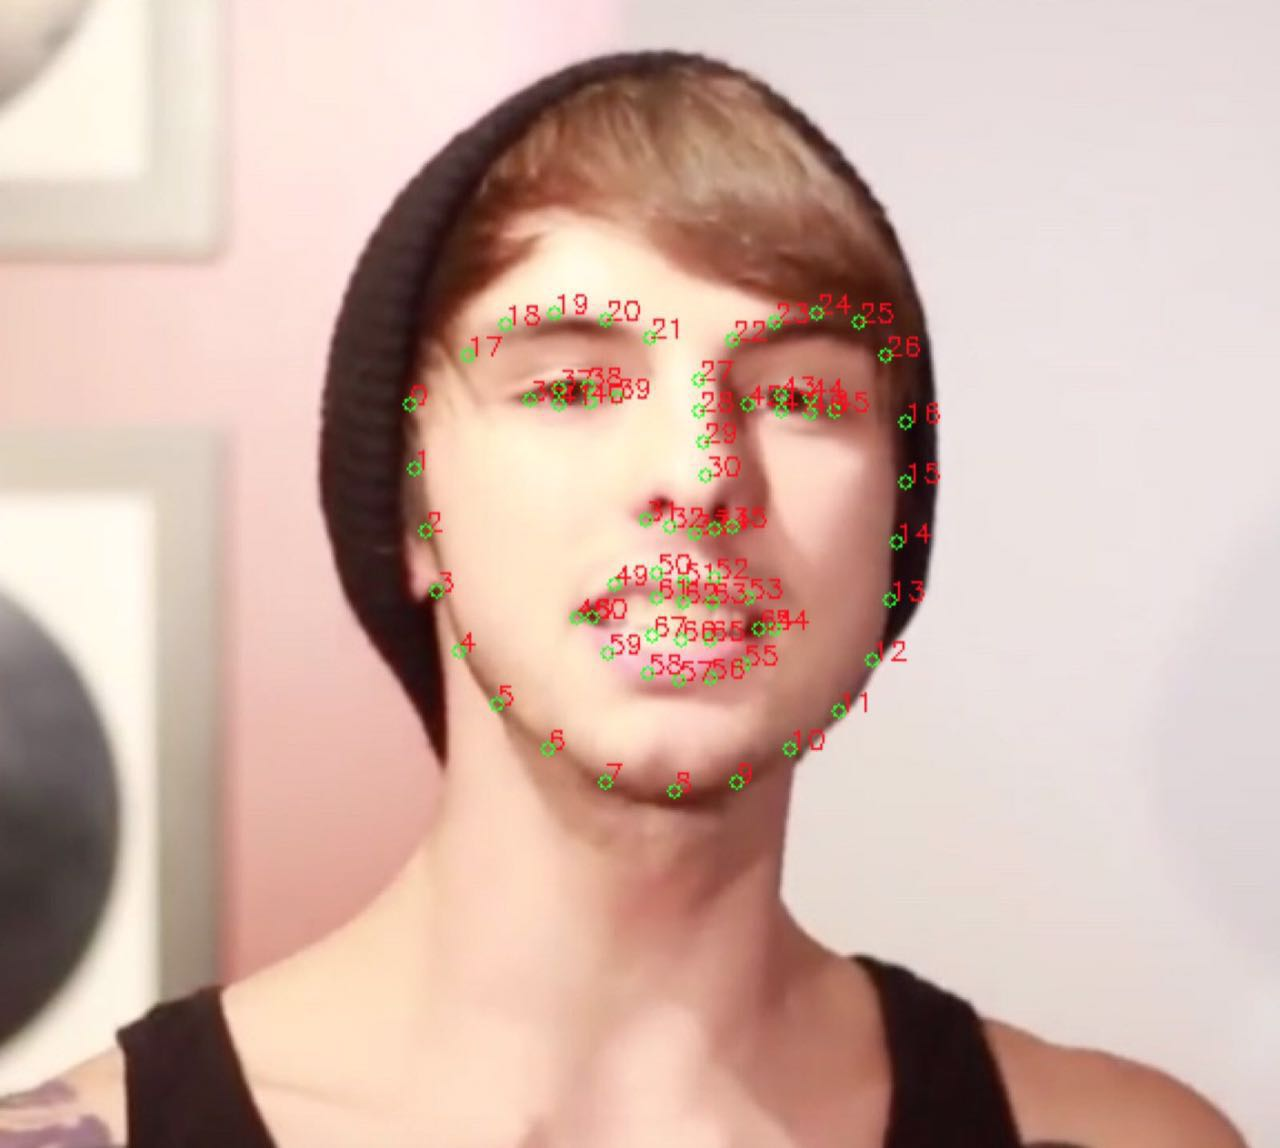
\includegraphics[width=0.5\linewidth]{images/face68.jpg}
\label{img:face68}
\end{center}
\item Adapt the affine transform into frames

Speaker in this picture has a frontal face to the camera, but it still has many faces can be detected with 68 landmarks but they only have side-face to the camera. Therefore, the affine transform is needed to normalize the impact of different head poses. In order to perform the affine transform, we set a landmark template, which is calculated by average frontal face landmarks in AV Lombard Grid corpus[6]. And then we compute the transform with RANSAC fitting algorithm.
\item Extract the ROI

The ROI is a fix-sized bounding box based on the coordinates of outer lip landmarks. Because the height and width are set by 1.2 multiply (max(x)-min(x)) and (max(y)-min(y)) of  these lip landmarks. Even though the size of bounding box is fixed, they’re only fixed in the same utterance of video. Therefore, we can extract the ROI and they are in RGB pixels.

\item Perform a 2d-dct on the ROI pixels to compress the frames information and remove correlation.

Before this, it is also necessary to rescale ROI on each frame to a fixed size of 240 by 240 and convert RGB vectors into YUV color space. Finally, we set the number of max feature count as 55, and then do the diagonal scanning on DCT matrix in order to achieve the 2 dimensional dct feature with 55 elements.

\end{enumerate}

\subsection{Video feature fusion with kaldi format}

To convert video feature into Kaldi’s format, we need to know what format the feature data present in the Kaldi. Kaldi has its script called make\_mfcc.sh can generate the mfcc feature and we can check the format with Kaldi’s binary file called copy-feats. Here is the mfcc feature and cmvn\_mfcc feature of the former 2 frames in utterance F002\_002\_01\_0101.00.001, as we can see, every frame has 13 vectors.
\begin{center}
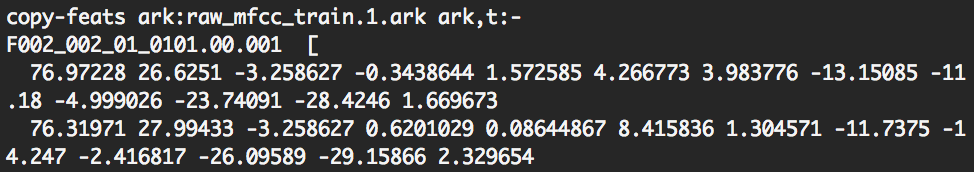
\includegraphics[width=1\linewidth]{images/train_mfcc.png}\\
\label{img:mfcc}
\end{center}
The cmvn\_mfcc feature is generated by running the script in kaldi called compute\_cmvn\_stats.sh in order to make mfcc features robust to some linear filtering of the signal. 
\begin{center}
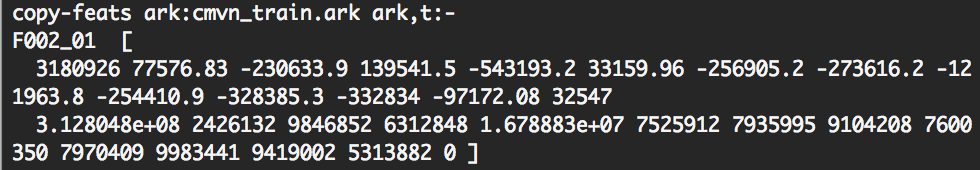
\includegraphics[width=1\linewidth]{images/cmvn_mfcc.png}\\
\label{img:cmvnmfcc}
\end{center}
The next step is to transfer video feature’s vectors with mfcc Kaldi’s format. The images below show the video feature vectors of the same utterance 
F002\_002\_01\_0101.00.001.
\begin{center}
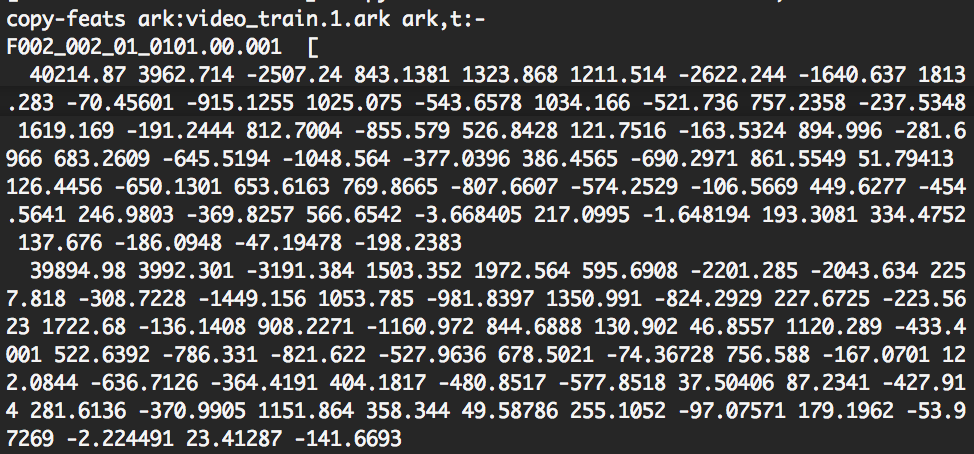
\includegraphics[width=1\linewidth]{images/train_video.png}\\
\label{img:video}
\end{center}

\begin{center}
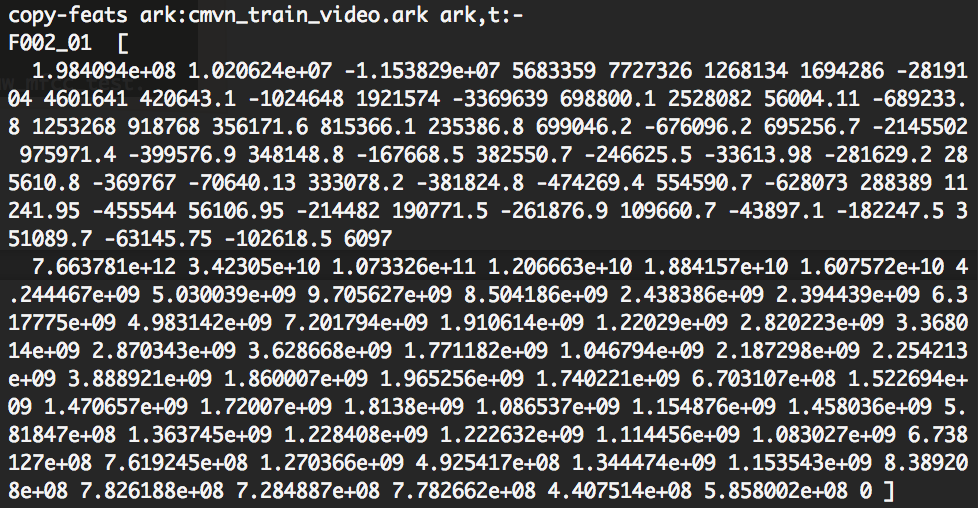
\includegraphics[width=1\linewidth]{images/cmvn_video.png}\\
\label{img:cmvnvideo}
\end{center}

\subsection{Generate Language model}
Since Kaldi is based on WFST framework, it provide tools to make standard arpa format represented as fst. In our recipes, we need to install and build the IRSTLM toolkit and use that to build language models from raw text.
In our project, we would generate uni-gram, bi-gram and tri-gram language model, and use them respectively to decode different acoustic models.
\subsection{ Train Acoustic models }
Training acoustic models with HMM-GMM method is a process of updating the parameters of HMM and GMM. In this project, we would use a few of Kaldi's scripts like train\_mono.sh, train\_deltas.sh, and train\_lda\_mllt.sh to train the acoustic models.
And the detailed steps of training acoustic models can be stated as follows:
\begin{enumerate}
\item Initialize GMM and output o.ml and tree file.
\item Compile training graphs and output fits.JOB.gz with o.mdl, tree and L.fst as input files.
\item Align the text annotation with frames with bin/align-equal-compiled binary file.
\item Do Maximum likelihood estimate on states which are based on GMM with gmmbin/gmm-est and get the parameter of GMM.
\item Iterate the process.
\item Accumulate the states based on GMM and do Maximum likelihood estimate  again to get the most likely sequence of states.
\item Merge the Maximum likelihood estimate results and generate the .mdl file.
\item Increase the number of guassians. If not surpass the number of iteration, return to the step 5 to train again.
\item Generate the final.mdl file as system's acoustic model.
\end{enumerate}

\subsection{Decode}
In this section, we need decode the training data with a suitable language model matching the trained acoustic model and then create the decoding graphs. For G.fst is a presentation of language model, L.fst is a presentation of lexicon dictionary, C.fst represents the context-dependent information and H.fst represents HMM, the process of decoding is to build a Transducer from the substate of context-dependent phoneme to word with viterbi algorithm.

\subsection{Evaluation methodology}

The most common way of evaluating an ASR system is to calculate the WER. To the specific AV-ASR system in music, there are also some specific methods to evaluate the system’s performance. For example, considering of the characteristics of different instrument, the effect degree to singing voice should be different as well. Therefore, we can separate songs by the type of accompanied-instrument and group them into different folders to exploit the effect of different instrument. Similar methods like pitch, tempo modification with dataset, also can be effect the audio-only ASR system's performance. For videos, we also can group songs into different folders according to the quality of video frames. Sometimes, the Lip region is partly sheltered from microphone or the frame has no face to be detected, any of them can reduce the performance of results. 

On the other hand, not in terms of modifying the input data. We can update the system's WER by adjusting the phone type of acoustic model and the size of n-gram language models. 






\chapter{Experimental results}
These experimental results are shown the different performances when adapting mfcc feature in Audio-only ASR system and adapting video feature in Visual-only ASR system. As the tables below,it is clear to see, even both of the WERs are over 90\%, the audio-only system still has better performance than visual-only ASR system.
\begin{table}[ht]
\center
\begin{tabular}{c|c|c|c}

Model & Uni-gram & Bi-gram & Tri-gram\\ \hline
Mono &93.58\% &91.76\% & 92.68\%\\ 
Tri1 &92.94\% &91.77\% & 92.09\%\\ 
Tri2b &94.03\% &91.60\% & 93.02\% \\ 
Tri3b &92.39\% &90.22\% & 90.74\%\\ 
\end{tabular}
\caption{WER of Audio-only ASR system}
\label{tab:AWER}
\end{table}

\begin{table}[ht]
\center
\begin{tabular}{c|c|c|c}

Model & Uni-gram & Bi-gram & Tri-gram\\ \hline
Mono &98.49\% &98.82\% & 99.06\%\\ 
Tri1 &99.29\% &99.58\% & 99.67\%\\ 
Tri2b &99.58\% &99.48\% & 99.48\% \\ 
\end{tabular}
\caption{WER of Visual-only ASR system}
\label{tab:VWER}
\end{table}
Mono model is a model that using an mono-phone acoustic model to train features. While tri1 model use tri-phone acoustic model to train dynamic features with deltas + delta-delta, tri2b model use tri-phone acoustic model to train dimensional reduced features that handled by LDA and MLLT transformations. Tri3b is a Speaker Adapted Training, therefore, we don't train visual feature with this process.   
And to analyze these two tables respectively, we can see that the WERs are generally lower in Audio-only ASR system when they are adapted with bi-gram language model to decode. While in terms of Visual-only ASR system, we can not make any conclusion to connect the WER results with the n-gram language model. However, they are clear to show the effects of the acoustic models. No matter decode with any n-gram language model here, the WERs in the mono-phone acoustic model are usually lower than tri-phone model. 

Tri-phone models are context-dependent phone models, we adapt them because in different situations, even the same phoneme has different pronunciation.But among visual features, this problem does not exist and that make sense why visual-only system performs better when training with mono phone model.

\section{Analysis of Visual-only ASR system's result}
The experimental results are too bad with over 98\% WER, that is even worse than the audio-only ASR system. Audio features are not pure because it contains noise and instrument sound. In terms of visual-only ASR system, the bad result may arise from the quality of extracted features or the limited size of music corpus. To verify the assumptions, the following sections would analyze them.

\subsection{analysis of extracted visual pixel features}
As we know, the feature extraction is an vital step in ASR systems based on statistic models. The quality of the extracted features may have heavy impacts on the decoding result. In this section, we would plot the extracted visual pixel features to see whether they are in good quality.

From these continuous frames in utterance: F002\_002\_01\_0101.00.001, they are clear to show the lip\_region information.
\begin{center}
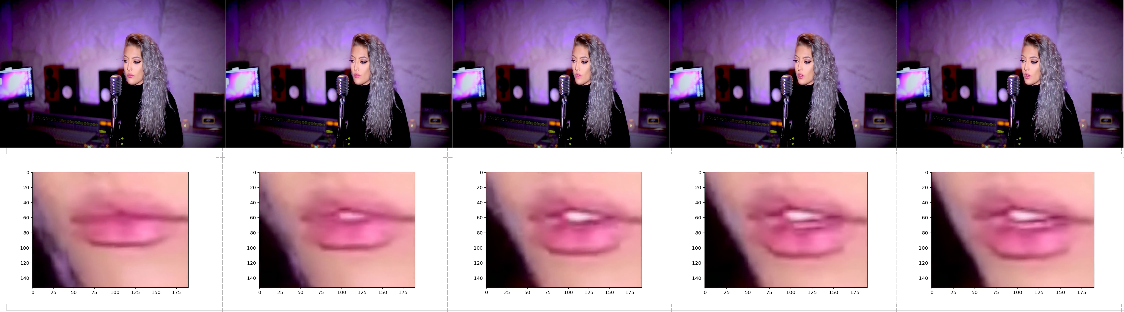
\includegraphics[width=0.8\linewidth]{images/F002.jpg}\\[1cm]
\label{img:F002}
\end{center}

However, the most extracted features\cite{2}} are not as good as the features above.
For example, in utterance : M020\_132\_01\_0101.00.027, the speaker moves his face quickly. As a result, the bounding box did not cover the ROI sometimes.
\begin{center}
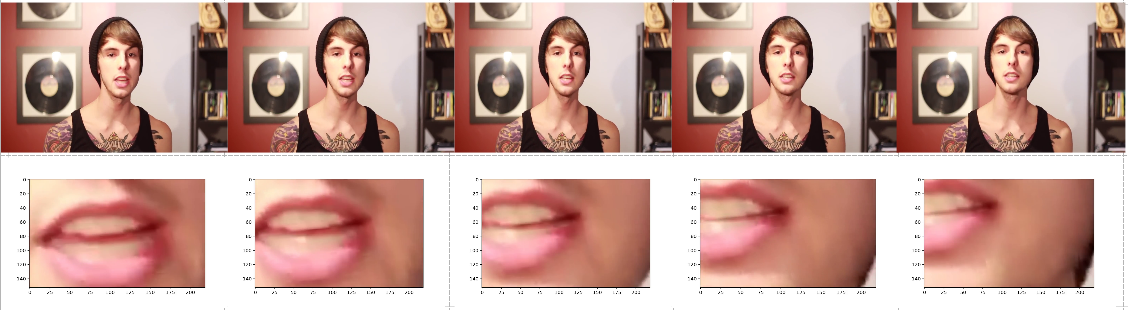
\includegraphics[width=0.8\linewidth]{images/M020.jpg}\\[1cm]
\label{img:M020}
\end{center}
In the following example, utterance-id : M001\_101\_01\_0101.00.022.
The extracted ROI features are bad because of the shelter of microphone.
\begin{center}
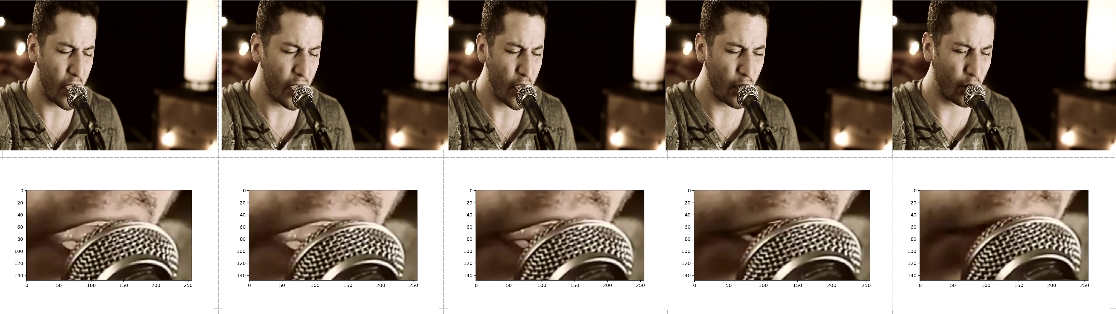
\includegraphics[width=0.8\linewidth]{images/M001.jpg}\\[1cm]
\label{img:M001}
\end{center}
While in this utterance M001\_001\_01\_0101.00.002 , the extracted features are more bad, since regardless of the shelter, the resolution of the video is low and may not able to show enough useful information.
\begin{center}
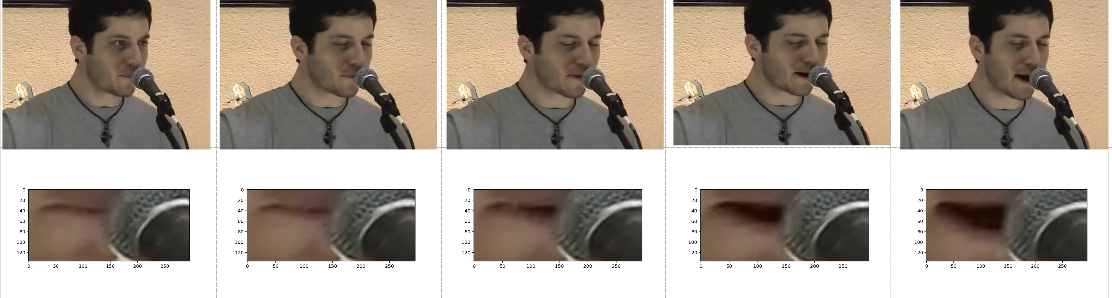
\includegraphics[width=0.8\linewidth]{images/M001_001.jpg}\\[1cm]
\label{img:M001_001}
\end{center}
Among these features, there is still another situation occurs in utterance M099\_044\_01\_0101.00.005. 
\begin{center}
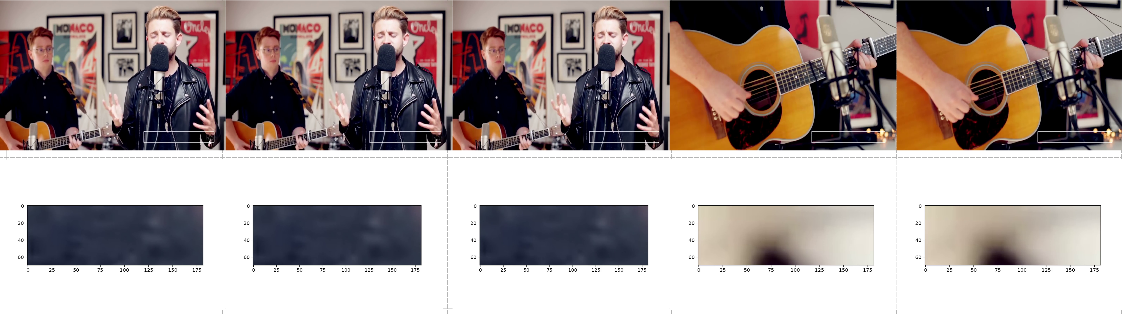
\includegraphics[width=0.8\linewidth]{images/M099.jpg}\\[1cm]
\label{img:M099}
\end{center}
The face detector in dlib toolkit mistaken the microphone as the detected face, and extract the part of it as lip region.
\begin{center}
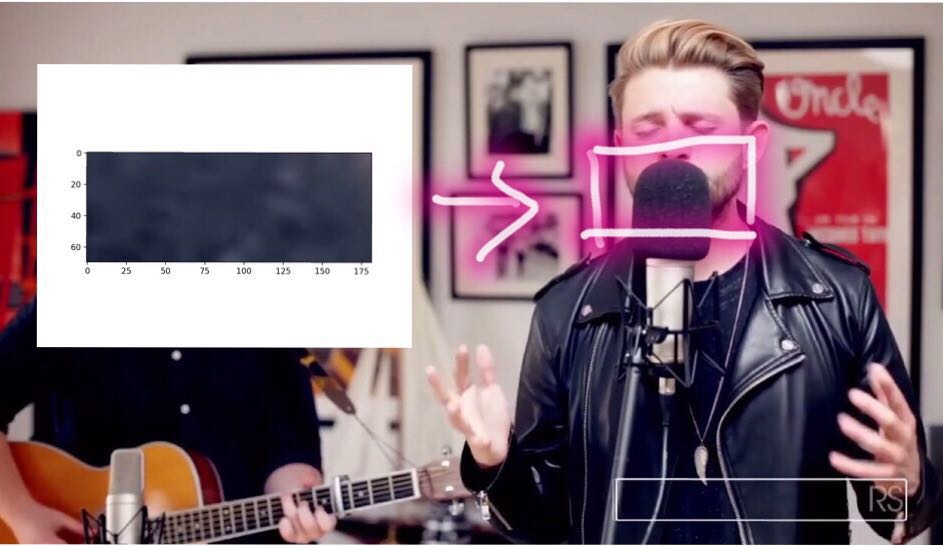
\includegraphics[width=0.6\linewidth]{images/bad1.jpg}\\[1cm]
\label{img:bad1}
\end{center}
\begin{center}
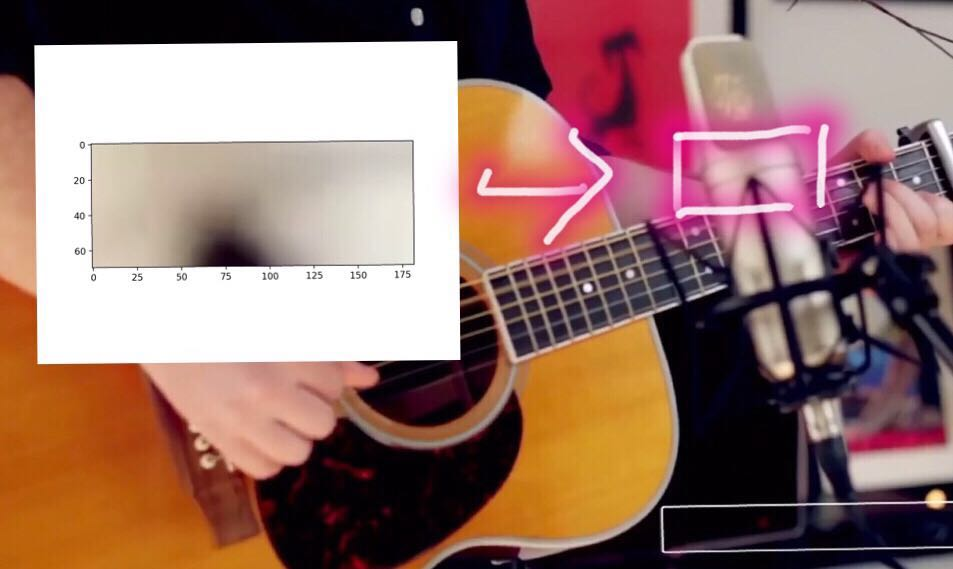
\includegraphics[width=0.6\linewidth]{images/bad2.jpg}\\[1cm]
\label{img:bad2}
\end{center}
The bad extracted features shown above may explain the reason why we got such bad WER results in visual-only ASR systems to some extent. To test whether the extracted features are still help in training the classifier. We
take the training set data also as the testing set and get the following results.
\begin{table}[ht]
\center
\begin{tabular}{c|c}

Model & WER\\ \hline
Mono &85.28\% \\ 
Tri1 &79.19\% \\ 
Tri2b &70.38\% \\ 

\end{tabular}
\caption{WER of Visual-only ASR system with training and testing on the same data set}
\label{tab:AWER}
\end{table}
This result is indeed a improvement and it reveals that the extracted visual features are still useful in training models.
\subsection{analysis of the size of music corpus}
As the table \ref{tab:utterance} shows, we just picked up 1013 utterances as a mini video corpus to build the visual-only ASR system. And among them only 615 utterances are for training , the left 398 utterances are taken as the testing set. Even though the WER results of Visual-only ASR system are more bad than Audio-only ASR system. We should notice that the audio-only ASR systems were trained and tested with 3428 utterances in total. Therefore, it is not reasonable to confirm which system performs better.


In the future, we should extend the useful video corpus in order to improve the Visual-only ASR system. Moreover, the algorithm of estimating lip region still can be improved, we should also focus on how to extract accurate visual features.

\section{Bad lip reading}

\textbf{Bad Lip Reading} is a YouTube channel,work to recompose films, TV shows, songs, sports, and political news stories by overdubbing humorous vocal that matches the lip movements of targets. It shows that, even audio-only front end system is weak in robust noise, visual-only front end system is also not reliable. Here are two videos, one is the original MV called \textbf{'you\'re beautiful'} from famous singer \textbf{James Blunt}, and the other is from this channel.
 
 These two videos\cite{3}} can be obtained on the website and the address would be appended in the following appendix. 




\section{Conclusion}
No matter ' lip reading for song transcription' or ' audio-only ASR in music', it is difficult to achieve results with low WER. For systems those already been built, it is hard to confirm whether the audio-only ASR system performs better or not, due to the different size of training data set.And in terms of visual-only ASR system, it could have a great improvement by extending the music corpus with good quality video files in extracting features. In the future, we can also focus on combing the audio front end with the visual front end to develop an AV-ASR system to see the performance.

\bibliographystyle{acm} 
\bibliography{mybibliography} 

\begin{appendices}
\chapter{Details of experimental result}

Detail of the insertions, deletions and substitutions words
\begin{table}[ht]
\center
\begin{tabular}{c|c|c|c|c|c}

Uni-gram   & Model & total words& Insertions & Deletions & Substitutions \\ \hline
           & Mono &  2121   &14 &1468 & 607\\ 
           &Tri1 &   2121   &3 &1673 & 430\\ 
           &Tri2b&  2121   &2 &1817 & 293 \\ \hline
Bi-gram   & Model & total words& Insertions & Deletions & Substitutions \\ \hline
           & Mono &  2121   &10 &1467 & 619\\ 
           &Tri1 &   2121   &5 &1494 & 613\\ 
           &Tri2b&  2121   &1 &1858 & 251 \\ \hline
Tri-gram   & Model & total words& Insertions & Deletions & Substitutions \\ \hline
           &Mono &  2121   &14 &1370 & 717\\ 
           &Tri1 &   2121   &4 &1476 & 634\\ 
           &Tri2b&  2121   &2 &1785 & 323 \\ \hline

\end{tabular}
\caption{Detail of the insertions, deletions and substitutions words of Visual-only ASR system}
\label{tab:DV}
\end{table}

\begin{table}[ht]
\center
\begin{tabular}{c|c|c|c|c|c}


Bi-gram   & Model & total words& Insertions & Deletions & Substitutions \\ \hline
           & Mono &  4008   &29 &2036 & 1353\\ 
           &Tri1 &   4008   &21 &2375 & 778\\ 
           &Tri2b&  4008   &1 &2320 & 500 \\ \hline

\end{tabular}
\caption{Detail of the insertions, deletions and substitutions words of Visual-only ASR system trained and tested by the same data set}
\label{tab:DV2}
\end{table}

\end{appendices}

\end{document}
